\documentclass{standalone}
\usepackage{tikz}
\usepackage{nono}
\begin{document}
  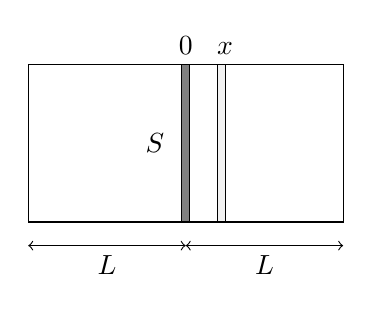
\begin{tikzpicture}
    \draw (0,0) rectangle (4,2);
    \draw[fill=gray] (1.95, 0) rectangle (2.05, 2);
    \draw (2, 2) node[above]{$0$};
    \draw[fill=gray!10] (2.4, 0) rectangle (2.5, 2) node[above]{$x$} ;
    \draw[<->] (0, -0.3) -- (2, -0.3) node[midway, below]{\(L\)}; 
    \draw[<->] (2, -0.3) -- (4, -0.3) node[midway, below]{\(L\)}; 
    \draw (1.85, 1) node[left]{\(S\)};
  \end{tikzpicture}
\end{document}
